\documentclass[11pt, twocolumn]{article}
\usepackage[margin=1.8cm, top=1.5cm, bottom=1.5cm]{geometry}
\usepackage{amsmath, amssymb}
\usepackage{graphicx}
\usepackage{booktabs}
\usepackage{hyperref}
\usepackage{caption}
\usepackage{float}
\usepackage{enumitem}
\setlist{nosep, leftmargin=*}

\captionsetup{font=small, labelfont=bf}
\setlength{\columnsep}{0.6cm}

\title{\vspace{-1.5cm}\textbf{Linear Regression: Gradient Descent vs.\ Closed-Form OLS}\\[4pt]
\large Mathematics for Machine Learning --- Final Project}
\author{Albert School $\times$ Mines Paris PSL}
\date{May 2026}

\begin{document}
\maketitle
\vspace{-0.5cm}

\section{Introduction}

We implement linear regression from scratch on the Ames Housing dataset (1,460 homes, 79 features) using two approaches: \textbf{batch gradient descent} (GD) and the \textbf{closed-form Normal Equation} (OLS). We select the top 10 numerical features by Pearson correlation, apply log-transformation to the target (reducing skewness from 1.88 to 0.12), and standardize features. The project integrates concepts from all five course sessions: eigendecomposition and PCA (S1), gradient computation and optimization (S2), distribution analysis (S3), hypothesis testing (S4), and regularization (S5).

\section{Mathematical Framework}

\subsection{Cost Function \& Gradient}

We minimize the Mean Squared Error:
\begin{equation}
J(\boldsymbol{\theta}, b) = \frac{1}{2n} \|\mathbf{X}\boldsymbol{\theta} + b\mathbf{1} - \mathbf{y}\|_2^2
\end{equation}

The gradient with respect to $\boldsymbol{\theta}$ is:
\begin{equation}
\nabla_{\boldsymbol{\theta}} J = \frac{1}{n} \mathbf{X}^T(\mathbf{X}\boldsymbol{\theta} + b\mathbf{1} - \mathbf{y})
\end{equation}

\subsection{Gradient Descent Update}

Parameters are updated iteratively:
\begin{equation}
\boldsymbol{\theta}_{t+1} = \boldsymbol{\theta}_t - \alpha\,\nabla_{\boldsymbol{\theta}} J(\boldsymbol{\theta}_t)
\end{equation}
Convergence requires $0 < \alpha < 2/\lambda_{\max}(\mathbf{X}^T\mathbf{X}/n)$.

\subsection{Normal Equation}

Setting $\nabla J = 0$ directly yields:
\begin{equation}
\boldsymbol{\theta}^* = (\tilde{\mathbf{X}}^T\tilde{\mathbf{X}})^{-1}\tilde{\mathbf{X}}^T\mathbf{y}
\end{equation}
where $\tilde{\mathbf{X}} = [\mathbf{1} \mid \mathbf{X}]$ is the augmented design matrix.

\section{Results}

\subsection{Convergence Analysis}

After standardization, $\kappa(\mathbf{X}^T\mathbf{X}/n) = 50.1$ with $\lambda_{\max} = 5.27$, giving a theoretical maximum learning rate of $\alpha < 0.38$.

\begin{figure}[H]
\centering
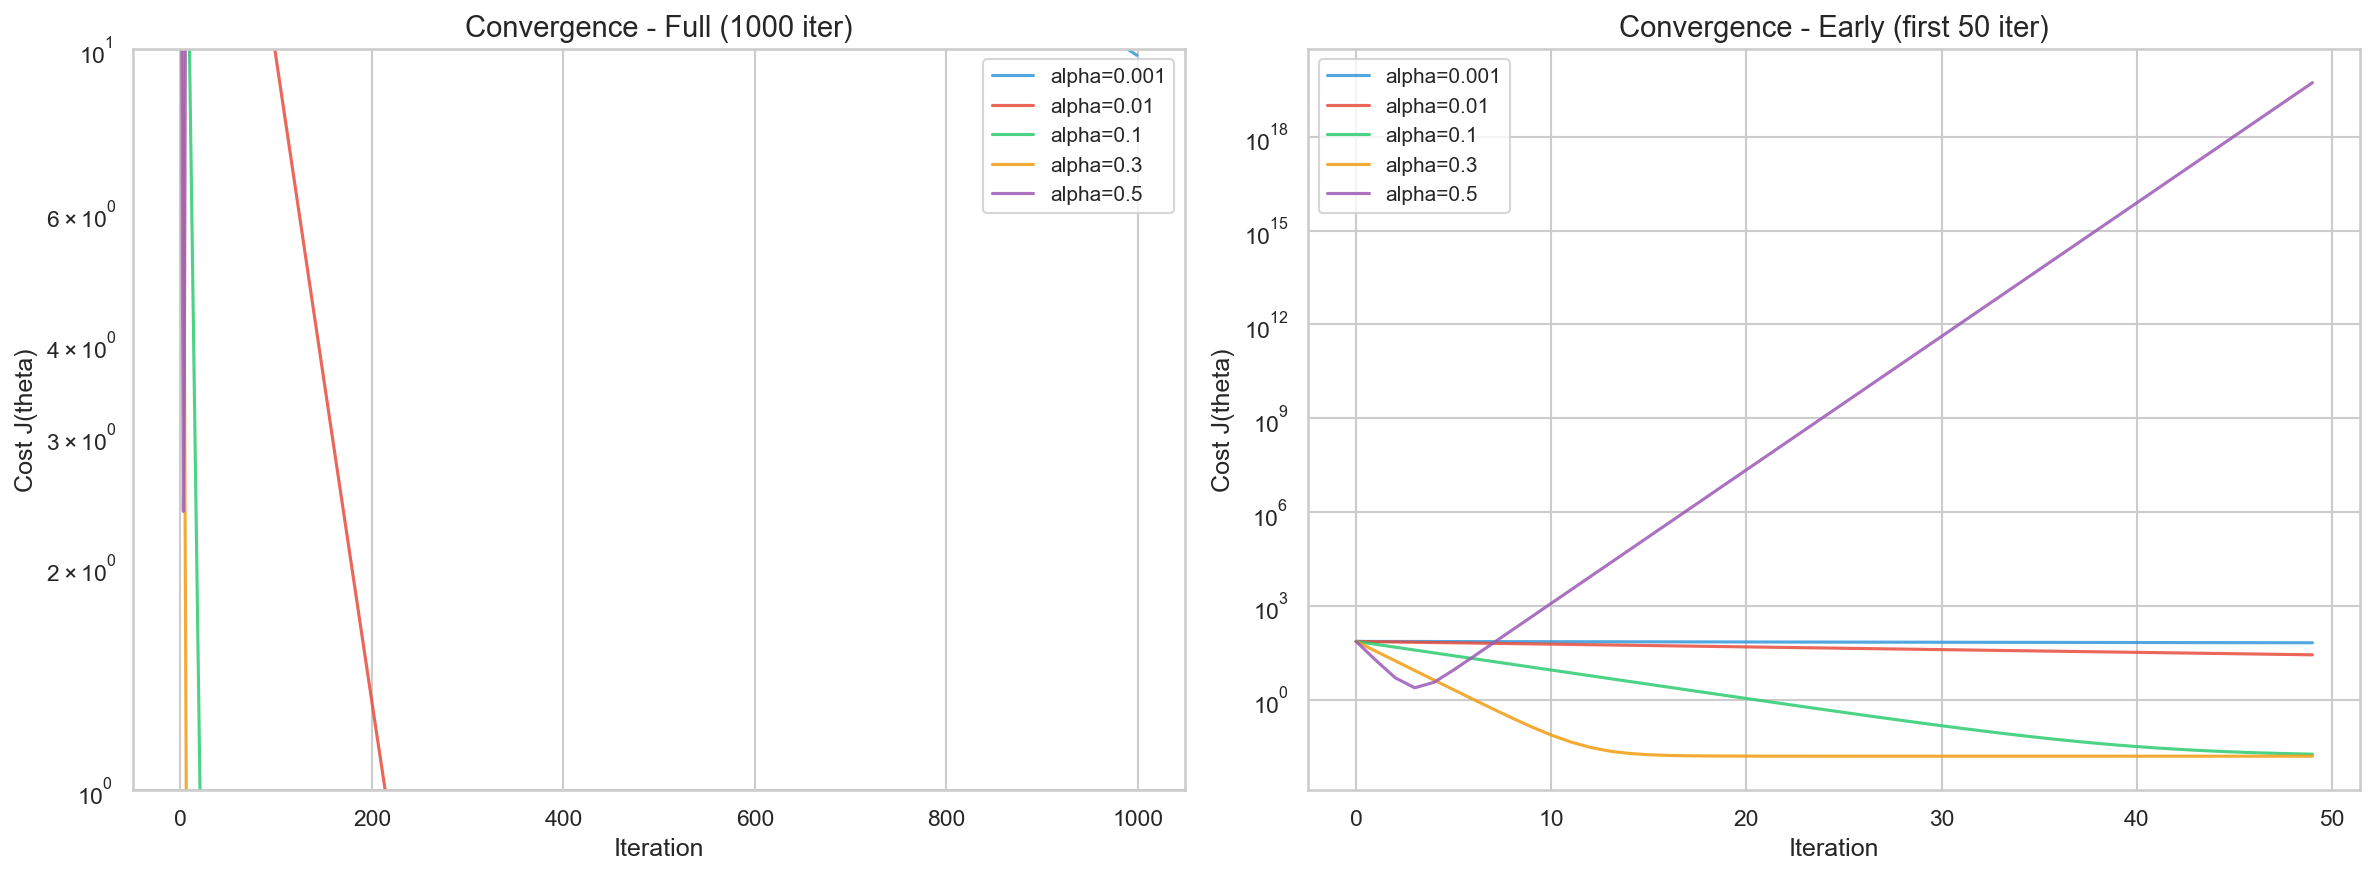
\includegraphics[width=\linewidth]{fig_learning_rates.png}
\caption{Convergence across learning rates. $\alpha=0.1$ and $0.3$ converge quickly; $\alpha=0.001$ barely moves in 1000 iterations; $\alpha=0.5$ diverges (exceeds the theoretical bound).}
\label{fig:lr}
\end{figure}

With $\alpha = 0.1$ and $T = 1000$, GD matches OLS to $\max|\theta_{\text{GD}} - \theta_{\text{OLS}}| = 10^{-6}$.

\subsection{Performance Comparison}

\begin{table}[H]
\centering
\small
\caption{OLS vs.\ Gradient Descent ($\alpha = 0.1$, $T = 1000$)}
\begin{tabular}{lcc}
\toprule
\textbf{Metric} & \textbf{OLS} & \textbf{GD} \\
\midrule
Train RMSE & 0.1758 & 0.1758 \\
Test RMSE & 0.1413 & 0.1413 \\
Train $R^2$ & 0.8132 & 0.8132 \\
Test $R^2$ & 0.8528 & 0.8528 \\
Time (ms) & 0.30 & 23.44 \\
\bottomrule
\end{tabular}
\end{table}

Both methods achieve identical performance ($R^2 = 0.853$ on the test set). OLS is ${\sim}78\times$ faster for this problem size ($p = 10$), but GD scales better to high-dimensional settings and naturally extends to regularization.

\subsection{Statistical Analysis}

A Welch's $t$-test confirms that overall quality ($\geq 7$ vs.\ $< 7$) significantly affects sale prices ($p \approx 0$), validating OverallQual as the most predictive feature ($r = 0.79$).

\section{Free Exploration}

\subsection{PCA (Session 1)}

Eigendecomposition of the feature covariance matrix reveals that 7 of 10 principal components capture 96\% of total variance. Regression on these 7 PCs achieves $R^2 = 0.843$ (vs.\ 0.853 with all features), demonstrating effective dimensionality reduction with minimal performance loss.

\subsection{Ridge Regularization (Session 5)}

We extend GD by adding an $L_2$ penalty: $J_{\text{Ridge}} = J + \frac{\lambda}{2n}\|\boldsymbol{\theta}\|^2$. Increasing $\lambda$ progressively shrinks weights toward zero. For this dataset, moderate regularization ($\lambda \leq 10$) maintains $R^2 \approx 0.85$, while strong regularization ($\lambda = 100$) reduces $\|\boldsymbol{\theta}\|_2$ by 9\% with only a slight $R^2$ decrease to 0.847.

\section{Conclusion}

Gradient descent converges to the exact OLS solution when the learning rate respects the spectral bound $\alpha < 2/\lambda_{\max}$. Feature standardization is essential---it reduces the condition number and enables convergence. PCA achieves 30\% dimensionality reduction with $<1.2\%$ $R^2$ loss, and Ridge regularization offers a natural extension of GD for complexity control. The project demonstrates how linear algebra (eigendecomposition), calculus (gradient computation), probability (distributional analysis), statistics (hypothesis testing), and optimization (GD, regularization) form an integrated mathematical toolkit for machine learning.

\end{document}
